\documentclass[11pt]{article}

% ============================================================================
% Jaravi — Documento de estrategia de producto y arquitectura
% Compilar con: xelatex jaravi.tex  (dos pasadas para referencias/enlaces)
%
% Nota de motor: el bootstrap de ConTeXt LMTX en C:\Users\USER\context solo
% trae mtxrun.exe (el instalador de red nunca se completó — requiere
% descargar la distribución completa desde mirrors). XeLaTeX/MiKTeX está
% instalado y verificado en esta máquina (tikz, tcolorbox, fontspec con
% fuentes del sistema), y da el mismo control de diseño absoluto que pedía
% la prueba original de ConTeXt, así que este documento usa XeLaTeX.
% ============================================================================

\usepackage{fontspec}
\setmainfont{Constantia}
\setsansfont{Corbel}
\setmonofont{Consolas}

\usepackage[a4paper,margin=2.4cm,top=2.6cm,bottom=3cm]{geometry}
\usepackage{xcolor}
\usepackage{tikz}
\usetikzlibrary{shapes.geometric,arrows.meta,positioning,fit,backgrounds,calc}
\usepackage{booktabs}
\usepackage{tabularx}
\usepackage[most]{tcolorbox}
\usepackage{titlesec}
\usepackage{fancyhdr}
\usepackage{enumitem}
\usepackage{microtype}
\usepackage[para]{footmisc}
\usepackage{xspace}

% ---- paleta (continuidad visual con el Dashboard WPF de Jaravi) -----------
\definecolor{jaravinavy}{HTML}{1E1E2E}
\definecolor{jaravipanel}{HTML}{181825}
\definecolor{jaraviaccent}{HTML}{7C6CF0}
\definecolor{jaravigreen}{HTML}{4CAF50}
\definecolor{jaraviamber}{HTML}{FFB300}
\definecolor{jaravired}{HTML}{E53935}
\definecolor{jaravimuted}{HTML}{5C6370}
\definecolor{jaravipaper}{HTML}{FAFAFC}
\definecolor{jaravirule}{HTML}{D8D8E3}

\usepackage[colorlinks=true,linkcolor=jaraviaccent,citecolor=jaraviaccent,urlcolor=jaraviaccent,pdftitle={Jaravi: Orquestacion Determinista de Sub-Agentes de IA},pdfauthor={Jaravi}]{hyperref}

\pagecolor{white}

% ---- tipografía de secciones ------------------------------------------------
\titleformat{\section}
  {\normalfont\sffamily\Large\bfseries\color{jaravinavy}}
  {\textcolor{jaraviaccent}{\thesection}}{0.5em}{}
  [\vspace{-0.3em}{\color{jaravirule}\titlerule[0.8pt]}]
\titleformat{\subsection}
  {\normalfont\sffamily\large\bfseries\color{jaravinavy}}
  {\textcolor{jaraviaccent}{\thesubsection}}{0.5em}{}
\titlespacing*{\section}{0pt}{1.6em}{0.8em}
\titlespacing*{\subsection}{0pt}{1.2em}{0.5em}

\pagestyle{fancy}
\fancyhf{}
\renewcommand{\headrulewidth}{0.4pt}
\renewcommand{\footrulewidth}{0pt}
\fancyhead[L]{\small\sffamily\color{jaravimuted} Jaravi --- Orquestacion determinista de sub-agentes}
\fancyhead[R]{\small\sffamily\color{jaravimuted} \thepage}
\fancyfoot[C]{\small\sffamily\color{jaravimuted} Documento interno de estrategia --- julio 2026}

\setlist[itemize]{leftmargin=1.4em,itemsep=0.2em,topsep=0.3em}
\setlist[enumerate]{leftmargin=1.6em,itemsep=0.2em,topsep=0.3em}

% ---- cajas de estadística grande -------------------------------------------
\newtcolorbox{statbox}[2]{
  colback=jaravipaper, colframe=jaravirule, boxrule=0.6pt, arc=3pt,
  width=#2, halign=center, valign=center, boxsep=4pt,
  before skip=4pt, after skip=4pt,
  fonttitle=\sffamily\bfseries,
}
\newcommand{\stat}[3][jaraviaccent]{%
  \begin{minipage}[t]{#2}
    \centering
    {\sffamily\bfseries\fontsize{22}{24}\selectfont\color{#1}#3}\\[2pt]
  \end{minipage}%
}

% ---- callout (nota / advertencia) -----------------------------------------
\newtcolorbox{callout}[2][jaraviaccent]{
  enhanced, breakable, colback=white, colframe=#1!70!black,
  boxrule=0pt, leftrule=3pt, arc=1pt, outer arc=1pt,
  colbacktitle=white, coltitle=#1!60!black,
  fonttitle=\sffamily\bfseries\small,
  title={#2}, attach title to upper, before upper={\par\vspace{2pt}},
  left=10pt, right=8pt, top=6pt, bottom=6pt,
}

\newcommand{\jaravi}{\textsc{Jaravi}\xspace}

% ============================================================================
\begin{document}
\sloppy

% ---- portada ----------------------------------------------------------------
\begin{titlepage}
\begin{tikzpicture}[remember picture, overlay]
  \fill[jaravinavy] (current page.north west) rectangle ([yshift=-8.6cm]current page.north east);
  \fill[jaraviaccent] ([yshift=-8.6cm]current page.north west) rectangle ([yshift=-8.68cm]current page.north east);
\end{tikzpicture}

\vspace{2.2cm}
\begin{flushleft}
\hspace{2cm}
\begin{minipage}{0.85\textwidth}
{\color{white}\sffamily\bfseries\fontsize{40}{44}\selectfont Jaravi}\\[6pt]
{\color{jaraviaccent!80!white}\sffamily\Large El jefe determinista de tus agentes de IA}\\[4pt]
{\color{white!70!jaravinavy}\sffamily\small Orquestacion, gobierno y control de costos para sistemas multiagente}
\end{minipage}
\end{flushleft}

\vspace{3.6cm}
\begin{center}
\begin{minipage}{0.8\textwidth}
\centering
{\sffamily\large\bfseries\color{jaravinavy} Documento de estrategia de producto y arquitectura}\\[8pt]
{\sffamily\color{jaravimuted} Version 0.3 --- Julio 2026}
\end{minipage}
\end{center}

\vfill
\begin{center}
{\sffamily\small\color{jaravimuted}
Motor: .NET 8 / C\# \quad$\bullet$\quad Protocolo: Model Context Protocol (MCP) \quad$\bullet$\quad Licencia propuesta: MIT (open-core)
}
\end{center}
\vspace{1cm}
\end{titlepage}

\tableofcontents
\thispagestyle{empty}
\newpage

% ============================================================================
\section{Resumen ejecutivo}

\jaravi es un motor de orquestacion \emph{determinista} que convierte a un agente de IA de alto nivel (Claude Code, o cualquier cliente MCP) en el jefe de un equipo de sub-agentes externos --- OpenCode, Codex CLI, Claude Code headless, GitHub Copilot CLI, Antigravity --- sin que la conversacion del jefe colapse por el volumen de logs, y sin pagar el sobrecosto de tokens que implica usar un LLM para decidir cada paso de la orquestacion.

La investigacion de mercado 2026 confirma que este es exactamente el cuello de botella que estanca la adopcion empresarial de sistemas multiagente: el \textbf{60\% de los pilotos de IA multiagente no llegan a produccion}, y la causa citada con mas frecuencia es la \textbf{complejidad de orquestacion}\footnote{Deloitte, 2025, citado en Viston.tech, ``Multi-Agent Orchestration Challenges Enterprises Must Solve in 2026''.}. \jaravi ataca ese cuello de botella con una decision de arquitectura simple: el motor que decide cuándo lanzar, esperar, encolar o matar un sub-agente esta escrito en C\# determinista, no en un prompt. El LLM solo entra para decidir \emph{qué} delegar --- nunca para orquestar \emph{cómo}.

\begin{center}
\stat{0.24\textwidth}{60\%}\hfill
\stat[jaravigreen]{0.24\textwidth}{500}\hfill
\stat[jaraviamber]{0.24\textwidth}{97M}\hfill
\stat[jaravired]{0.24\textwidth}{15$\times$}
\end{center}
\vspace{-8pt}
\begin{center}
\footnotesize\sffamily\color{jaravimuted}
\begin{minipage}{0.24\textwidth}\centering pilotos multiagente que no llegan a producción\end{minipage}\hfill
\begin{minipage}{0.24\textwidth}\centering líneas de log máx.\ por lectura en \jaravi (tope duro)\end{minipage}\hfill
\begin{minipage}{0.24\textwidth}\centering descargas/mes de los SDKs de MCP (mar-2026)\end{minipage}\hfill
\begin{minipage}{0.24\textwidth}\centering sobrecosto de tokens de la orquestación vía LLM\footnotemark\end{minipage}
\end{center}
\footnotetext{Estimado por Anthropic para arquitecturas multiagente orquestadas por LLM; citado en analisis de mercado 2026 sobre costos de sistemas agenticos.}

% ============================================================================
\section{El problema: colapso de contexto y explosión de costos}

Tres investigaciones independientes de 2026 describen el mismo problema desde ángulos distintos, y los tres describen exactamente lo que \jaravi fue diseñado para resolver.

\subsection{Colapso de contexto silencioso}
En flujos de trabajo largos, el contexto acumulado llena la ventana del agente orquestador; cuando se acerca al límite, el modelo \textbf{empieza a descartar instrucciones anteriores en silencio} --- incluyendo restricciones críticas\footnote{FlowHunt, ``Multi-Agent AI Systems in 2026: What the Research Actually Says''.}. Con cuatro o más trabajadores, el contexto excede la ventana con frecuencia. No es un fallo visible: el agente sigue respondiendo, pero con reglas que ya no recuerda.

\begin{callout}[jaraviaccent]{Cómo lo resuelve Jaravi}
El motor absorbe \emph{todo} el output de los subprocesos en un ring buffer acotado por sesión. El jefe nunca recibe más de 500 líneas por lectura (tope duro server-side, configurable pero nunca desactivable), y el patrón recomendado es leer \texttt{get\_summary} --- un digest de exit code, duración y errores extraídos --- en vez de logs crudos. Verificado en pruebas: una sesión que emitió 50{,}002 líneas devolvió exactamente 500 en la lectura.
\end{callout}

\subsection{Explosión de costos}
Las herramientas agénticas cuestan entre \$200 y \$2{,}000+ por ingeniero al mes en gasto de tokens, y los sistemas multiagente multiplican ese costo: cada agente de un equipo de cinco consume tokens de forma independiente. Flujos que cuestan \$0.50 en pruebas pueden llegar a \$50{,}000/mes en producción a 100{,}000 ejecuciones, porque el orquestador hace múltiples llamadas al LLM solo para descomponer y agregar tareas, encima de cada llamada de los trabajadores\footnote{KGT Solutions, ``Multi-Agent AI Orchestration: A CTO's 2026 Guide''.}.

\begin{callout}[jaravired]{Cómo lo resuelve Jaravi}
\jaravi nunca invoca un LLM para decidir el \emph{cómo} de la orquestación --- spawn, await, cola, kill son código C\# determinista, con costo de cómputo, no de tokens. El jefe (el único LLM en el ciclo) paga tokens solo por decidir \emph{qué} delegar y por leer resúmenes acotados. La tool \texttt{run\_agent} colapsa el patrón spawn+await+summary en una sola llamada MCP, reduciendo también las rondas de ida y vuelta del jefe.
\end{callout}

\subsection{La brecha de escalamiento}
El 80\% de las empresas que empiezan con un solo agente planean orquestar múltiples agentes en dos años, pero \textbf{menos del 10\% lo ha logrado}\footnote{Gartner, citado en Kanerika, ``AI Agent Orchestration in 2026: What Enterprises Need to Know''.}. Sin coordinación, gobierno y observabilidad, los agentes duplican trabajo, producen resultados inconsistentes y crean puntos ciegos de seguridad.

\begin{callout}[jaravigreen]{Cómo lo resuelve Jaravi}
\emph{Scope Gate} valida cada \texttt{workdir} contra raíces permitidas antes de lanzar un proceso. \emph{Claims} de rutas (v0.3) declaran qué sesiones pueden escribir dónde, con rechazo estructurado o cola FIFO automática --- elimina la duplicación de trabajo por diseño, no por instrucción. El Dashboard WPF da observabilidad en tiempo real vía WebSocket sin tocar el contexto del jefe.
\end{callout}

% ============================================================================
\section{El mercado}

\subsection{Tamaño y crecimiento}
\begin{table}[h]
\centering
\small
\begin{tabularx}{\textwidth}{X r r r}
\toprule
\textbf{Segmento} & \textbf{2024/25} & \textbf{2026} & \textbf{Proyección} \\
\midrule
Mercado de agentes de IA & \$5.25\,mil M & --- & \$52.62\,mil M (2030, CAGR 46.3\%) \\
Agentes autónomos & --- & \$8.5\,mil M & \$35\,mil M (2030) \\
Asistentes de código IA & --- & \$12.8\,mil M & \$30.1\,mil M (2032, CAGR 27\%) \\
Servicios open-source & --- & \$66.84\,mil M & --- \\
\bottomrule
\end{tabularx}
\caption{Tamaño de mercado y proyecciones, fuentes de investigación de mercado 2026 (ver referencias).}
\end{table}

Gartner proyecta que el 40\% de las empresas integrará agentes de IA hacia fines de 2026, y los CIOs esperan que para 2030 el 75\% del trabajo de TI involucre personas aumentadas con IA.

\subsection{MCP como estándar de facto}
El Model Context Protocol --- el protocolo que \jaravi habla nativamente --- ha cruzado de protocolo de nicho a infraestructura mainstream de agentes:

\begin{itemize}
\item \textbf{41\%} de las organizaciones de software encuestadas están en producción limitada o amplia con servidores MCP.
\item El registro oficial de MCP contaba \textbf{9{,}652} servidores únicos y \textbf{28{,}959} versiones al 24 de mayo de 2026.
\item Los SDKs de TypeScript y Python de MCP alcanzaron \textbf{97 millones} de descargas mensuales en marzo de 2026.
\item En diciembre de 2025, Anthropic donó MCP a la \emph{Agentic AI Foundation} (AAIF), un fondo dirigido bajo la Linux Foundation cofundado con Block y OpenAI --- consolidando a MCP como estándar neutral de proveedor.
\item El panorama se ha estabilizado en un modelo de dos capas: \textbf{MCP} para integración vertical con herramientas, \textbf{A2A} (Google) para coordinación horizontal entre agentes.
\end{itemize}

\subsection{El ecosistema de CLIs que Jaravi ya orquesta}
\begin{table}[h]
\centering
\small
\begin{tabularx}{\textwidth}{l X r}
\toprule
\textbf{Agente} & \textbf{Posición de mercado (jul-2026)} & \textbf{Perfil en Jaravi} \\
\midrule
OpenCode & Líder open-source: 180{,}312 estrellas en GitHub (MIT) & \texttt{opencode} \\
Codex CLI (OpenAI) & \#1 en Terminal-Bench 2.1, 83.4\% & \texttt{codex} \\
Claude Code & 46\% de satisfacción (JetBrains, abr-2026), 134{,}868 estrellas & \texttt{claude} \\
GitHub Copilot & Líder en adopción: 29\% uso laboral, 4.7M suscriptores pagos & \texttt{copilot} \\
Cursor & \$2\,mil M ARR, 1M+ usuarios de pago & \emph{(vía extensión de perfil)} \\
\bottomrule
\end{tabularx}
\caption{Cada fila es una entrada declarativa en \texttt{agents.json} --- cero cambios de código para agregar un nuevo CLI.}
\end{table}

% ============================================================================
\section{Arquitectura: motor determinista, no otro agente}

La decision de diseño central de \jaravi es que el \textbf{motor de orquestacion no es un agente de IA}. Es un programa .NET convencional con maquina de estados, colas y buffers --- exactamente el tipo de sistema que la ingenieria de software sabe hacer confiable, auditable y barato de correr. El unico LLM en el ciclo es el jefe, que habla con el motor por MCP.

\begin{center}
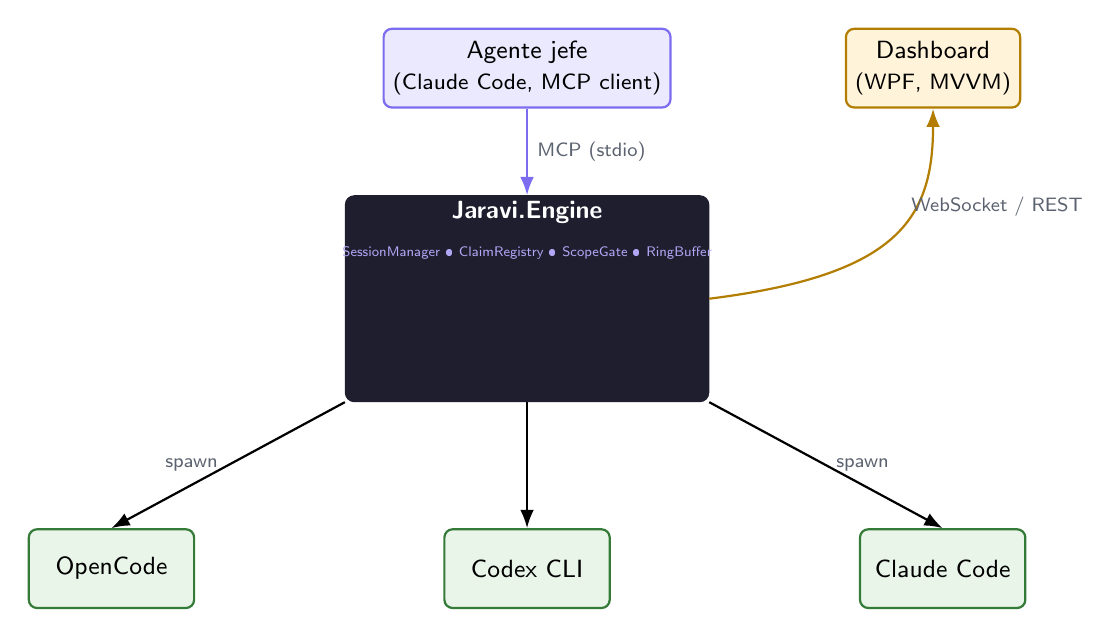
\begin{tikzpicture}[
  node distance=0.9cm and 1.6cm,
  box/.style={draw, rounded corners=3pt, thick, minimum height=1cm, align=center, font=\sffamily\small},
  boss/.style={box, fill=jaraviaccent!15, draw=jaraviaccent},
  engine/.style={box, fill=jaravinavy, text=white, draw=jaravinavy},
  agent/.style={box, fill=jaravigreen!12, draw=jaravigreen!70!black, minimum width=2.1cm},
  observer/.style={box, fill=jaraviamber!15, draw=jaraviamber!70!black},
  lbl/.style={font=\sffamily\scriptsize, color=jaravimuted},
  >=Latex
]

\node[boss] (boss) {Agente jefe\\\footnotesize(Claude Code, MCP client)};
\node[engine, below=1.1cm of boss, minimum width=4.6cm, minimum height=2.6cm] (engine) {};
\node[font=\sffamily\bfseries\small, text=white, above=0.05cm of engine.north, anchor=north] (enginelbl) {Jaravi.Engine};
\node[font=\sffamily\tiny, text=jaraviaccent!60!white, below=0.05cm of enginelbl] {SessionManager \textbullet\ ClaimRegistry \textbullet\ ScopeGate \textbullet\ RingBuffer};

\node[observer, right=2.2cm of boss] (dash) {Dashboard\\\footnotesize(WPF, MVVM)};

\node[agent, below left=1.6cm and 1.9cm of engine] (a1) {OpenCode};
\node[agent, below=1.6cm of engine] (a2) {Codex CLI};
\node[agent, below right=1.6cm and 1.9cm of engine] (a3) {Claude Code};

\draw[->, thick, jaraviaccent] (boss) -- node[lbl, right] {MCP (stdio)} (engine.north);
\draw[->, thick, jaraviamber!70!black] (engine.east) .. controls +(2.4,0.3) and +(0,-1.4) .. node[lbl, above right, pos=0.55] {WebSocket / REST} (dash.south);
\draw[->, thick] (engine.south west) -- node[lbl, left] {spawn} (a1.north);
\draw[->, thick] (engine.south) -- (a2.north);
\draw[->, thick] (engine.south east) -- node[lbl, right] {spawn} (a3.north);

\end{tikzpicture}
\end{center}

\begin{itemize}
\item \textbf{Jaravi.Core} --- dominio puro: modelos, eventos, contratos. Cero dependencias externas.
\item \textbf{Jaravi.Engine} --- el motor determinista: \texttt{SessionManager} (ciclo de vida y máquina de estados), \texttt{ClaimRegistry} (bloqueos de rutas), \texttt{ChannelEventBus} (telemetría sin bloqueo), \texttt{RingBufferLogStore} (logs acotados), \texttt{ScopeGate} (seguridad de \texttt{workdir}).
\item \textbf{Jaravi.McpServer} --- host Kestrel: 10 tools MCP, WebSocket de eventos, REST. Distribuido como \texttt{dotnet tool} global (\texttt{jaravi-mcp}) --- instalación de un comando, cero rutas absolutas en la configuración del cliente.
\item \textbf{Jaravi.Dashboard} --- observador WPF/MVVM, desacoplado del motor (solo consume HTTP/WebSocket). Nunca afecta al motor si se cierra.
\end{itemize}

% ============================================================================
\section{Diferenciación técnica}

\begin{table}[h]
\centering
\footnotesize
\begin{tabularx}{\textwidth}{X X X}
\toprule
\textbf{Capacidad} & \textbf{Frameworks orquestados por LLM} & \textbf{Jaravi} \\
\midrule
Decisión de spawn/wait/kill & Inferencia del LLM en cada paso & Máquina de estados determinista en C\# \\
Costo de orquestación & Tokens por cada decisión (``15$\times$ premium'') & Cómputo, no tokens \\
Colapso de contexto & Riesgo alto en sesiones largas & Ring buffer + tope duro de lectura (500 líneas) \\
Colisión de archivos entre agentes & Depende de la disciplina del prompt & \emph{Claims} declarativos con cola FIFO o rechazo \\
Encadenar resultados entre agentes & El jefe copia y pega manualmente & \texttt{inputFromSessionId} --- el motor inyecta el resultado \\
Agregar un nuevo CLI & Cambios de código / nuevo adaptador & Entrada declarativa en \texttt{agents.json} \\
Instalación & Script, Docker, o build manual & \texttt{dotnet tool install -g} --- un comando \\
\bottomrule
\end{tabularx}
\caption{Jaravi frente al patrón dominante de orquestación vía LLM.}
\end{table}

\subsection{Lo ya construido (v0.3, julio 2026)}
\begin{itemize}
\item \textbf{10 tools MCP}: \texttt{spawn\_agent}, \texttt{run\_agent} (spawn+await+summary en una llamada), \texttt{await\_session}, \texttt{get\_summary}, \texttt{read\_output} (acotado), \texttt{send\_input}, \texttt{kill\_agent}, \texttt{list\_agents}, \texttt{list\_sessions}, \texttt{get\_status}.
\item \textbf{Pipelines de sesiones}: encadena un agente auditor con un agente corrector sin que el jefe toque el resultado intermedio.
\item \textbf{Claims de rutas}: paralelismo seguro entre sub-agentes que escriben archivos.
\item \textbf{Distribución zero-friction}: \texttt{dotnet tool} global (\texttt{jaravi-mcp}), configuración de usuario auto-sembrada en \texttt{\%APPDATA\%\textbackslash jaravi}.
\item \textbf{54 pruebas automatizadas} (xUnit), incluyendo E2E contra procesos reales (timeout, kill, flood de 50k líneas, colas de claims).
\item \textbf{5 perfiles de CLI reales} verificados en producción: OpenCode, Codex, Claude Code, Copilot, Antigravity.
\end{itemize}

% ============================================================================
\section{Modelo de negocio: open-core}

El patrón validado para herramientas de desarrollador en 2026 es \emph{open-core}: núcleo libre que genera confianza, comunidad y distribución; capas comerciales para lo que las empresas exigen y los desarrolladores individuales no necesitan\footnote{GetMonetizely, ``Monetizing Open-Source Software: Pricing Strategies for Open-Core SaaS''; patrón validado por HashiCorp (Terraform) entre otros.}. Según la encuesta 2023 de OpenLogic, el \textbf{67\% de las empresas} que adoptan un producto open-core terminan pagando por el nivel superior.

\begin{table}[h]
\centering
\small
\begin{tabularx}{\textwidth}{l X X}
\toprule
& \textbf{Community (MIT, gratis)} & \textbf{Enterprise} \\
\midrule
Motor y tools MCP & Completo & Completo \\
Perfiles de agentes & \texttt{agents.json} local & Catálogo gestionado + plantillas verificadas \\
Dashboard & WPF de escritorio & Hosted, multi-usuario, multi-tenant \\
Gobierno & Scope Gate, claims locales & SSO/EMA, RBAC, políticas centralizadas \\
Auditoría & Eventos en memoria & Logs persistentes, exportación, retención \\
Soporte & Comunidad & SLA, cuenta dedicada \\
\bottomrule
\end{tabularx}
\caption{Propuesta de tiers, alineada con la extensión de Autorización Gestionada por Empresa (EMA) que el propio ecosistema MCP está estandarizando en 2026.}
\end{table}

Esta propuesta no es especulativa: la extensión \emph{Enterprise-Managed Authorization} de MCP --- ya en estado estable y adoptada por Asana, Atlassian, Canva, Figma, Linear y Supabase --- es exactamente el tipo de necesidad de gobierno que el tier Enterprise de \jaravi resolvería para el motor de orquestación.

% ============================================================================
\section{Roadmap}

\begin{enumerate}
\item \textbf{Ahora --- v0.3}: pipelines, claims, distribución como \texttt{dotnet tool}, 5 perfiles de CLI reales.
\item \textbf{Corto plazo}: \texttt{ConPtyIoStrategy} (PTY real) para CLIs que exigen TTY interactivo; persistencia NDJSON de logs por sesión; métricas de costo/uso por sesión y por perfil.
\item \textbf{Mediano plazo}: Dashboard hosted multi-usuario; integración EMA para gobierno centralizado; publicación del paquete en NuGet.org.
\item \textbf{Largo plazo}: puente A2A para coordinación horizontal con agentes no-CLI; catálogo público de perfiles verificados por la comunidad.
\end{enumerate}

% ============================================================================
\section{Conclusión}

El mercado de 2026 describe un problema preciso: las empresas quieren orquestar múltiples agentes de IA, pero el 60\% de los intentos fracasa por complejidad de orquestación, colapso de contexto y costos que escalan de forma impredecible. \jaravi responde con una tesis de ingeniería simple y verificable: \textbf{la orquestación no necesita inteligencia artificial, necesita determinismo}. El LLM decide qué hacer; un motor .NET convencional decide cómo hacerlo --- de forma auditable, barata y a prueba de colapso de contexto por diseño.

\vspace{1cm}
\begin{center}
{\sffamily\small\color{jaravimuted} --- fin del documento ---}
\end{center}

\newpage
\section*{Referencias}
\small
\begin{itemize}[leftmargin=1.2em]
\item Viston.tech (2026). \textit{AI Agent Orchestration in 2026: Enterprise Guide to Multi-Agent Systems}; \textit{Multi-Agent Orchestration Challenges Enterprises Must Solve in 2026}.
\item Kanerika (2026). \textit{AI Agent Orchestration in 2026: What Enterprises Need to Know}.
\item Deloitte (2025/2026). \textit{Unlocking exponential value with AI agent orchestration}.
\item KGT Solutions (2026). \textit{Multi-Agent AI Orchestration: A CTO's 2026 Guide}.
\item FlowHunt (2026). \textit{Multi-Agent AI Systems in 2026: What the Research Actually Says}.
\item Digital Applied (2026). \textit{MCP Adoption Statistics 2026: Model Context Protocol}.
\item InfoQ (2026). \textit{AI Model Context Protocol Adds Centralised Auth for Enterprise}.
\item Toloka AI (2026). \textit{The future of MCP: 2026 roadmap, enterprise adoption, and what comes next}.
\item Zylos Research (2026). \textit{Agent Interoperability Protocols 2026: MCP, A2A, ACP and the Path to Convergence}.
\item Morphllm (2026). \textit{Best AI Coding Agent (2026): Ranked by Terminal-Bench, Price, and Source}.
\item Ideaplan (2026). \textit{AI Coding Assistant Market Share 2026: Cursor vs Copilot}.
\item GetMonetizely (2026). \textit{Monetizing Open-Source Software: Pricing Strategies for Open-Core SaaS}.
\end{itemize}

\end{document}
